\subsection{Der spezifische Workflow}\label{l:workflow}

Hauptaufgabe der Anwendung ist es, den Workflow von der Definition bis zur Übernahmen der fertigen Texte in das Produkt zu übernehmen und dabei nicht nur Funktionen zur \emph{Definieren} und \emph{Speichern} und \emph{Exportieren} zu bieten, sondern auch die \emph{Kommunikation über die Texte} zu integrieren. Für die Umsetzung des Workflows in einer Anwendung müssen zunächst alle Ausprägungen der speziellen Abläufe beschrieben werden. In Abschnitt~\ref{l:besondererolle}~(S.\pageref{l:besondererolle}) wurde bereits beschrieben, wie umfangreich die Anzahl der Personen ist, die Einfluss auf die Texte eines Produktes haben. Die Rollenverteilung ist dabei von Projekt zu Projekt unterschiedlich, mit den in Abschnitt~\ref{l:personas}~(S.\pageref{l:personas}) vorgestellten Personas würde eine Übersicht über die typische Rollenverteilung geschaffen. 

\begin{table}
\begin{center}
\begin{tabular}{@{}r c c c}
\textbf{Persona} & \textbf{Inhalt} & \textbf{Attribute} & \textbf{Status}\\[1ex]
\textbf{Agentur} & & & \\
\hline\\[-1.5ex]
\emph{Eva}, Konzept & \HarveyQuarter & \HarveyFull & \HarveyEmpty \\
\emph{Lotte}, Art-Direktion & \HarveyEmpty & \HarveyThreeQuarters & \HarveyEmpty \\
\emph{Jan}, Produktion & \HarveyEmpty & \HarveyQuarter & \HarveyEmpty \\
\emph{Arthur}, Projektleitung & \HarveyEmpty & \HarveyEmpty & \HarveyQuarter \\[1ex]
\textbf{Extern} & & & \\
\hline\\[-1.5ex]
\emph{Torsten}, Text & \HarveyHalf & \HarveyEmpty & \HarveyEmpty \\
\emph{Jorinde}, Übersetzung & \HarveyQuarter & \HarveyEmpty & \HarveyEmpty \\[1ex]
\textbf{Kunde} & & & \\
\hline\\[-1.5ex]
\emph{Markus} & \HarveyHalf & \HarveyQuarter & \HarveyFull
\end{tabular}
\caption{Stärke des Einfluss, die Mitarbeiter in einem Projekt haben}
\label{table:texteinfluss}
\end{center}
\end{table}

Alle Mitarbeiter haben Einfluss auf drei grundlegenden Eigenschaften von Text:

\begin{enumerate}\itemsep -5pt
\item den \textbf{Inhalt} des Textes,
\item die \textbf{Attribute} wie z.B. \typoquotes{maximale Textlänge} oder \typoquotes{Position im Medium}
\item und den \textbf{Status} wie z.B. \typoquotes{neu} und \typoquotes{freigegeben}.
\end{enumerate}

Das Gewicht des Einfluss der Mitarbeiter ist je nach Rolle unterschiedlich, Tabelle~\ref{table:texteinfluss}~(S.\pageref{table:texteinfluss}) zeigt dies in einer Übersicht. 

\subsubsection{Einfluss auf den \textit{Inhalt}} 

Personen die Einfluss auf den \emph{Inhalt} haben, sind vor allem diejenigen die die Texte für das Produkt liefern. Neben den Mitarbeitern auf Kundenseite, Ausgangsmaterialien und Fachinformationen zur Verfügung stellen sind die Texter und Übersetzer, die diese Informationen aufbereitet. Texte müssen aber auch die die spezifischen Gegebenheiten des Mediums angepasst werden, hierzu liefern Experten Rahmenbedingungen aber auch inhaltliche Anpassungen. Ein Beispiel hierfür ist die suchmaschinenoptimierung (SEO) von Texten. Hierbei werden Texte auf das Vorhandensein von bestimmte Formulierungen und Stichwörter optimiert aber auch Vorgaben über die Länge und Aufbau von Texten gemacht. 

Mit Inhalt ist der eigentliche Text gemeint, der auch im Produkt erscheint. Für Inhalte gibt es immer eine Original-Version für die im späteren Projektverlauf Übersetzungen in eine oder mehrere Sprachen angelegt werden können. Die Übersetzung basiert dabei auf der Original-Version, oder je nach Übersetzer auch auf einer anderen Übersetzung.

Vorgaben für Inhalte werden in Form von Richtlinien formuliert. Diese Richlinen dienen dem Texter als Orientierungshilfe, wie er die Texte zu formulieren hat. Richtlinien werden von verschiedenen Mitarbeitern formuliert: 
\begin{itemize}\itemsep -5pt
\item Vom Konzept werden grundlegende Vorgaben geschaffen, wie z.B. Annahmen über die Zielgruppe und den Zweck des Produktes.
\item Der Kunde hat Vorstellungen oder sogar Vorgaben, wie die \typoquotes{Sprache} der Texte sein soll, aus seinen Fachabteilungen und von Beratern oder Anwälten werden weitere Vorgaben über erwünschte oder zu vermeidende Aussagen erstellt.
\end{itemize}
Es existieren aber auch implizite Vorgaben, die sich aus der Art des Mediums ergeben: Lange Texte sind für Fernsehspots ungeeignet, Informationsbröschüren haben Raum für ausführliche Erläuterungen.

Nicht selten werden weitere externe Experten zu Projekten hinzugezogen, die Texte auf bestimmte Aspekte hin anpassen. Besonders bei Internetseiten werden SEO-Konzepte erstellt, auf deren Basis die Texte von einzelnen Seiten und Abschnitten so angepasst werden, dass diese bestimmte Schlüsselwörter und Formulierungen enthalten, um von den Algorithmen der Suchmaschinenbetreiber bessere Positionierungen in Suchergebnissen zu erreichen.

\subsubsection{Einfluss auf die \textit{Attribute}} 

Attribute legen die Rahmenbedingungen von Text fest, diese werden vor allem in der Gestaltung des Produktes durch Designer, als auch in der Umsetzung durch produktbedingte Einschränkungen, z.B. Platzverhältnisse oder systembedingte Beschränkungen, bestimmt. 

\subsubsection{Einfluss auf den \textit{Status}} 

Den Status von Texten, also ob ein Text dem nächsten Mitarbeiter im Workflow zugewiesen werden soll kann von bestimmten Mitarbeitern abhängen. Es ist üblich, dass Texte erst dann dem Kunden zur Abnahme vorgelegt werden, wenn sie als Gesamtes vorliegen. Auch externe Dienstleister bekommen aus Kostengründen meisten alle Text im Paket, damit eine zügige Abarbeitung des Auftrages gewährleistet wird.

\TODO

\begin{figure}[htb]
\begin{center}
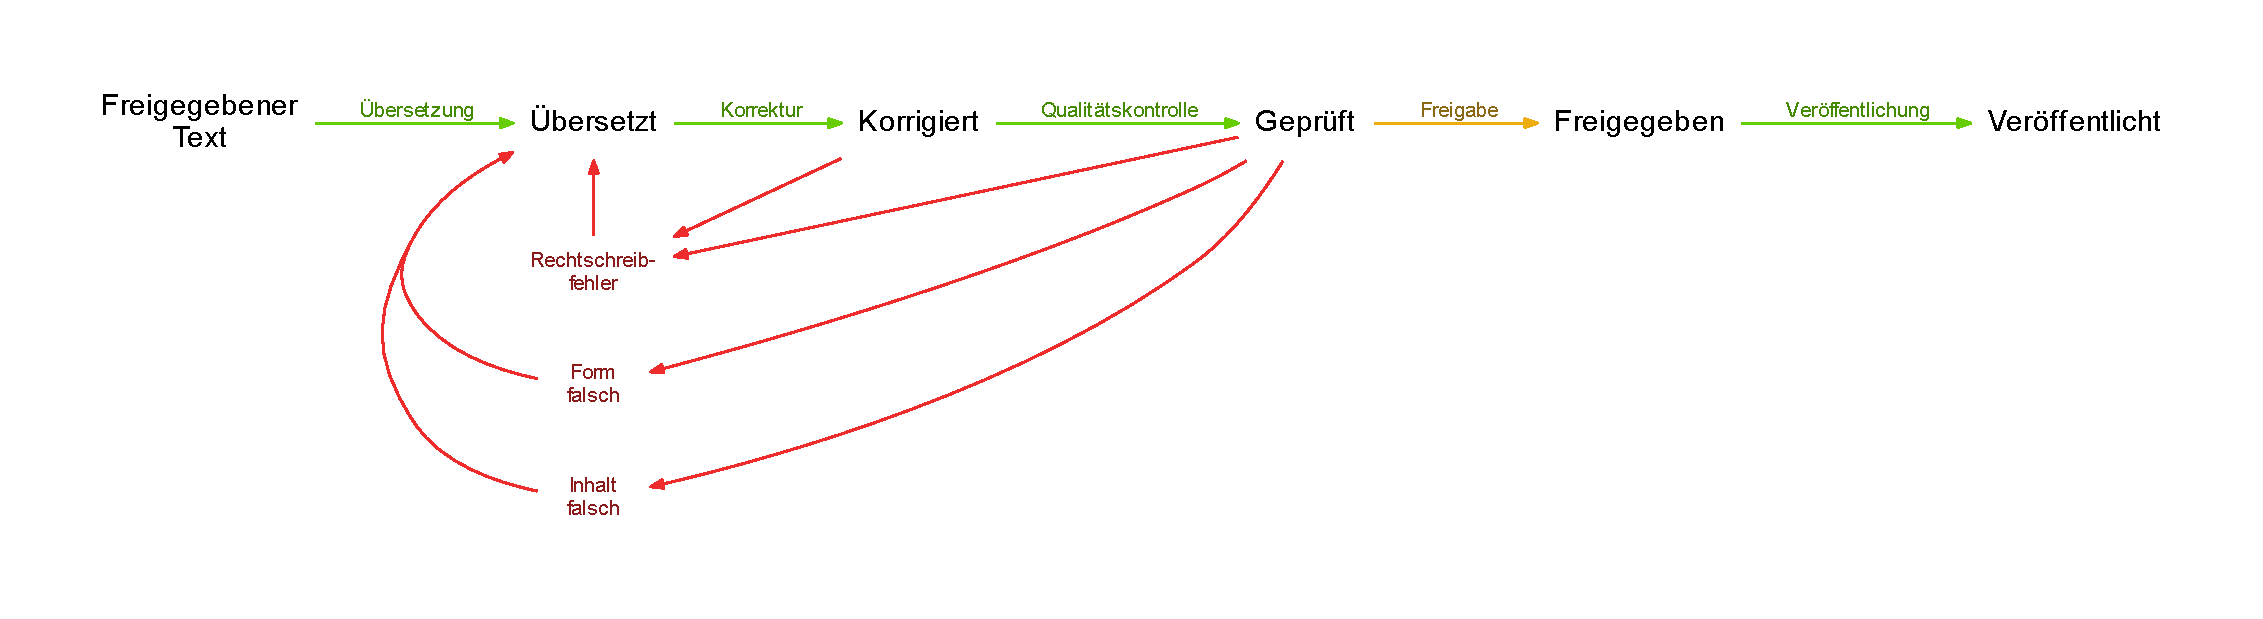
\includegraphics[width=\textwidth]{media/chart-5.pdf}
\end{center}
\caption{Operationen bei der Übersetzung von Texten mit Qualitätskontrolle}
\label{chart:5}
\end{figure}

Die bisher genannten Abläufe lassen sich auch 1:1 auf die Übersetzung von Texten anwenden. Abbildung~\ref{chart:5} zeigt den Workflow schematisch.

Abbildung~\ref{chart:personas-gewichtet}~(S.\pageref{chart:personas-gewichtet}) zeigt diese Beziehungen in einem, nach Anzahl der Kommunikationspartner gewichteten Graphen

\begin{figure}[htb]
\begin{center}
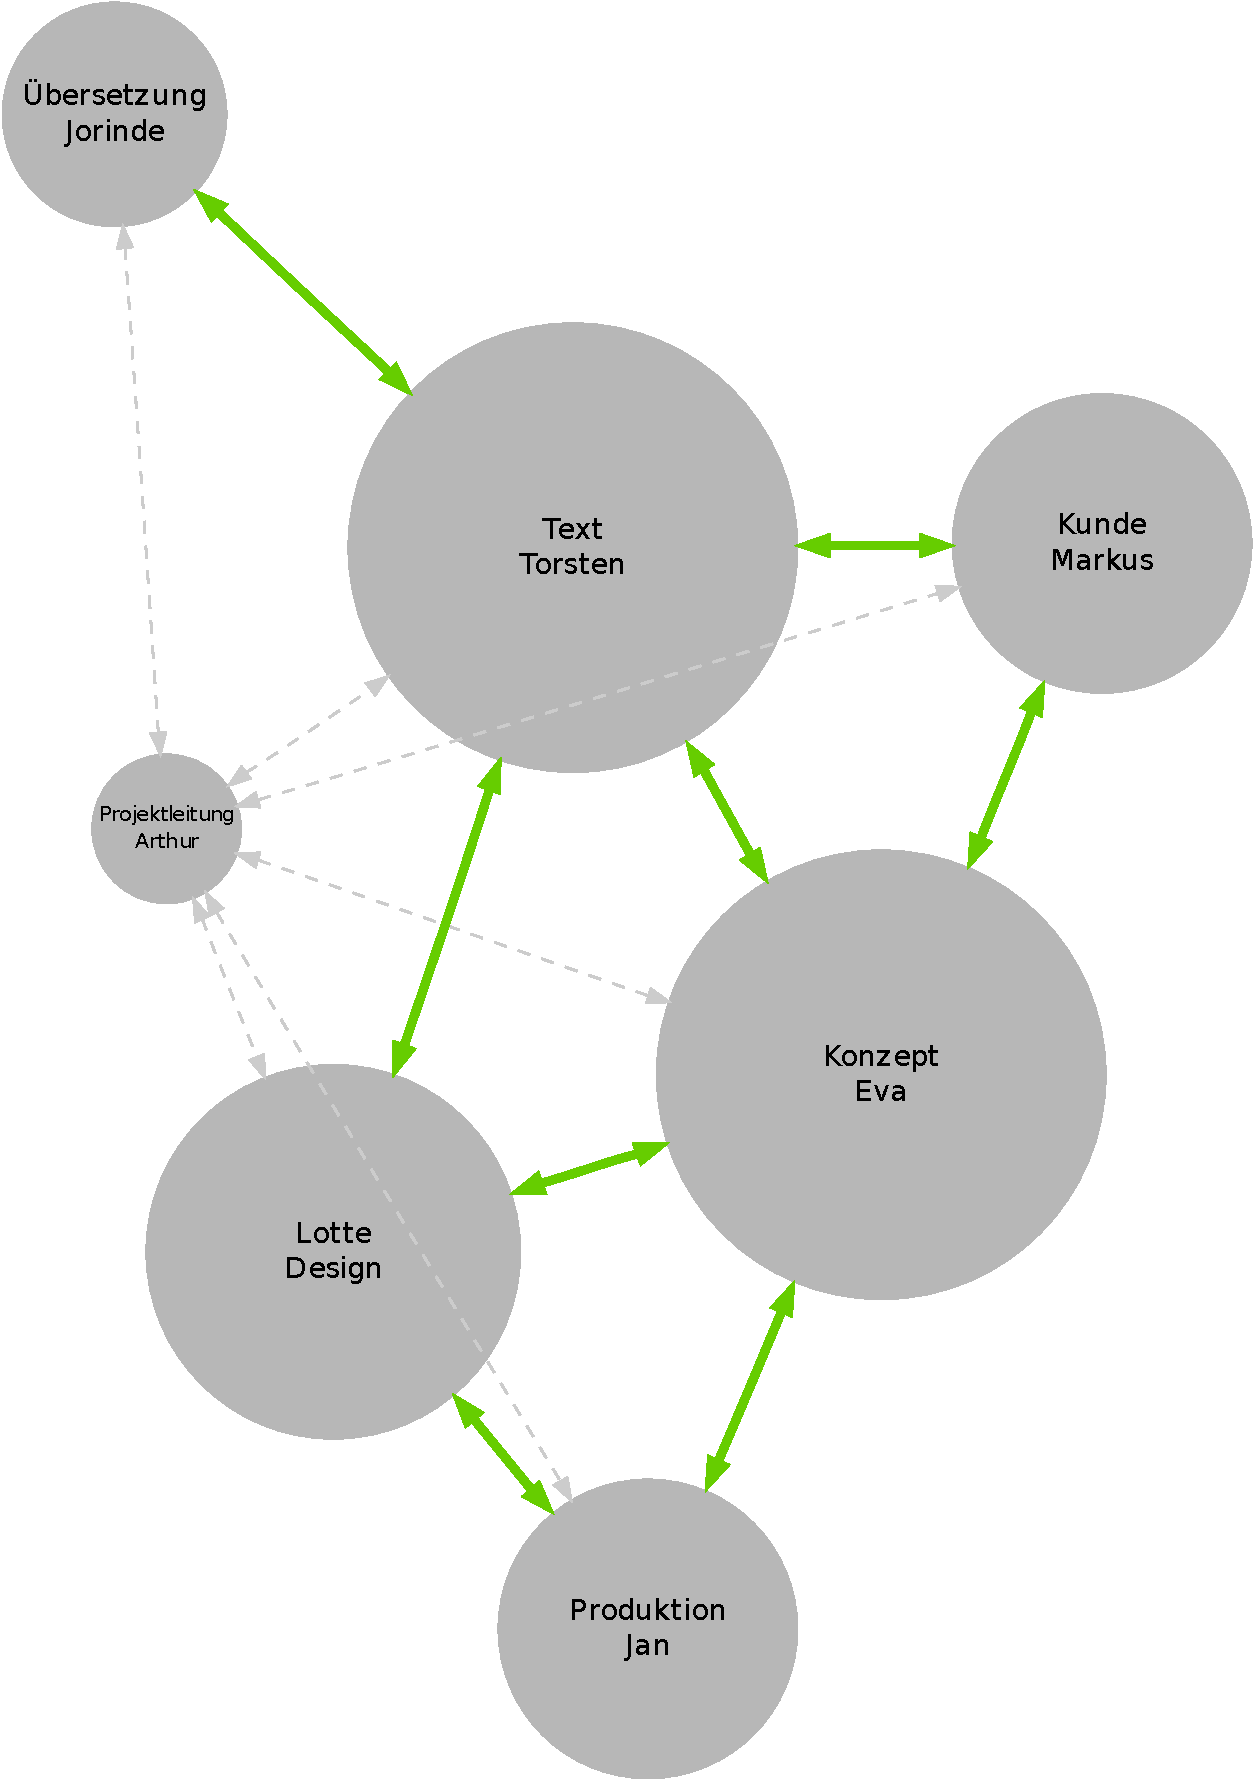
\includegraphics[width=0.85\textwidth]{media/personas-gewichtet.pdf}
\caption{Abstimmung zwischen den Personas bezogen auf Text, gewichtet nach Anzahl der Kommunikationspartner}
\label{chart:personas-gewichtet}
\end{center}
\end{figure}

\label{l:textattribute}

\paragraph{Typ} Überschrift, Untertitel, Bild-Beschreibung, Fließtext.

\paragraph{Workflow}

Beschreibung des optimalen Workflows und die Rolle der Beteiligten

Innerhalb der Anwendung wird das Projekt angelegt und die dafür benötigten Textbausteine definiert. Hierbei können detaillierte Angaben zu deren Eigenschaften gemacht werden, z.B. über den Verwendungszweck oder die maximal Länge. Die einzelnen Textbausteine werden bei diesem Vorgang entsprechend dem Aufbau des Endproduktes in eine Reihenfolge gebracht und hierarchisch angeordnet. So wird eine leichte Orientierung und Zuordnung der Text zum Endprodukt möglich. 

Nachdem die benötigten Textbausteine definiert wurden, werden diese durch Texter befüllt. Für Texter stellt die Anwendung Hilfsfunktionen zur Verfügung. Dazu zählen Informationen wie Zeichenlänge und Wortanzahl und Rechtschreibkorrektur mit Wörterbuch.

Sobald die Texte hinterlegt wurden durchlaufen sie die Qualitätskontrolle durch andere Mitarbeiter des Projektes und anschließend den Freigabeprozess beim Kunden. Wurden die Texte freigegeben, können die zusammengestellten Texte in das Endprodukt übernommen werden. 

Alle Vorgänge werden innerhalb der Anwendung protokolliert und sind so für jeden Beteiligten leicht nachvollziehbar. Aufgaben können automatisch aufgrund von Änderungen erzeugt werden, oder von Mitarbeiter angelegt werden. So wird sichergestellt, dass alle Projektmitarbeiter jederzeit über ihre Aufgaben bezüglich der Texte informiert sind, bei Änderungen die verantwortlichen Mitarbeiter informiert werden. Dadurch wird es möglich auch bei Korrekturen in letzter Minute diese Änderungen gezielt und transparent zu übernehmen.



% MARK


\begin{figure}[htb]
\begin{center}
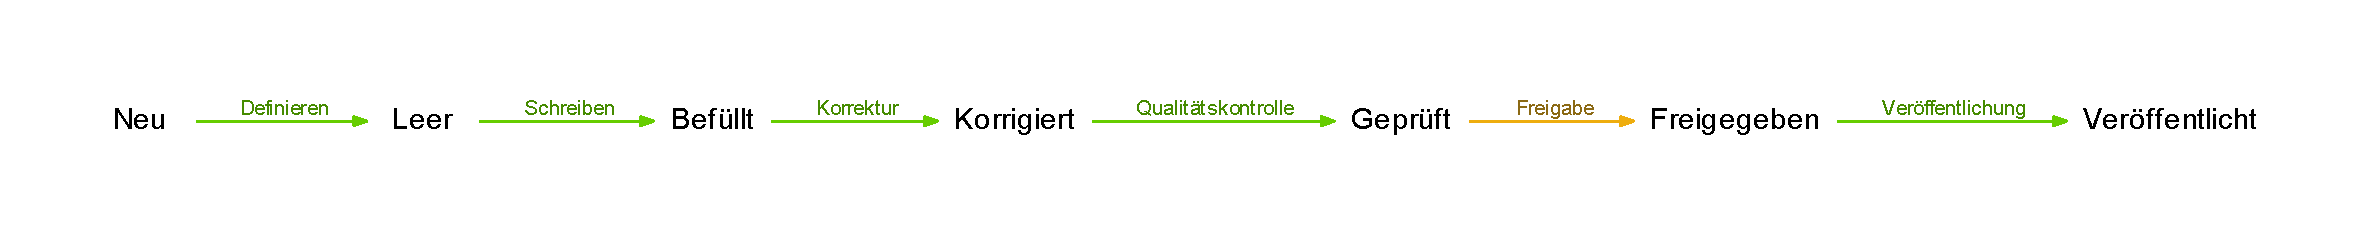
\includegraphics[width=\textwidth]{media/chart-3.pdf}
\end{center}
\caption{Operationen bei der Erstellung von Texten}
\label{chart:3}
\end{figure}

Betrachtet man die von Projektmitarbeitern durchgeführten Operationen in Zusammenhang mit Text lassen sich diese in sechs eigenständige Operationen unterteilen, die in Abbildung~\ref{chart:3}~(S.\pageref{chart:3}) in Zusammenhang dargestellt sind:

\begin{enumerate}
\item{Durch \textbf{Definieren eines Textbausteines} werden dessen \emph{Attribute} bestimmt. Dadurch wird festgelegt, wie der benötigte Text beschaffen sein muss. Die Aussage \citequotes{Wir brauchen an dieser Stelle eine Überschrift} ist ein Beispiel für diese Operation. Sie legt fest, wie der Textbausteine gestaltet werden muss, um die ihm zugedachte Aufgabe zu erfüllen. Neben der Angabe zur Platzierung auf dem Medium durch \typoquotes{an dieser Stelle} wird implizit durch \typoquotes{eine Überschrift} eine Angabe zur inhaltlichen und visuellen Gestaltung getroffen; Überschriften sollen kurz und knapp sein und ihre visuelle Gestaltung wird durch den Styleguide des Projektes festgelegt.}
\item{Das \textbf{Schreiben eines Textes} erzeugt den Inhalt eines Textbausteins in einer Sprache. Bei diesem Vorgang wird der Text entsprechend der Vorgabe aus der Beschreibung als Original erstellt oder aus Quellen außerhalb des Projektes kopiert und eingefügt. }
\item{In der \textbf{Korrektur} wird der Text inhaltlich und grammatikalisch überprüft und entsprechend angepasst. Der Korrektor muss dabei für eine grammatikalische Überprüfung des Textes kein Fachwissen bezogen auf das Projekt haben. Ist diese Fachwissen vorhanden, kann eine inhaltliche Korrektur vorgenommen werden.}
\item{In der \textbf{Qualitätskontrolle} wird der Text dahingehend überprüft, ob er den Anforderungen gemäß der Beschreibung und inhaltlichen Vorgaben, auch hinsichtlich des gesamten Projektes entspricht. Abbildung~\ref{chart:4} verdeutlicht den Einfluss der Qualitätskontrolle auf den Verlauf eines Projektes.}
\item{Durch die \textbf{Freigabe} wird der Text abgenommen und kann nun in das Endprodukt übernommen werden. Die Freigabe unterscheidet sich von der Qualitätskontrolle durch ihren authorativen Charakter. Qualitätskontrolle können prinzipiell von allen Mitarbeitern durchgeführt werden. Freigaben werden nur von Mitarbeitern mit Management-Berechtigungen erteilt.}
\item{Durch die \textbf{Veröffentlichung} wird der Text in das Endprodukt eingebracht.}
\end{enumerate}

\begin{figure}[htb]
\begin{center}
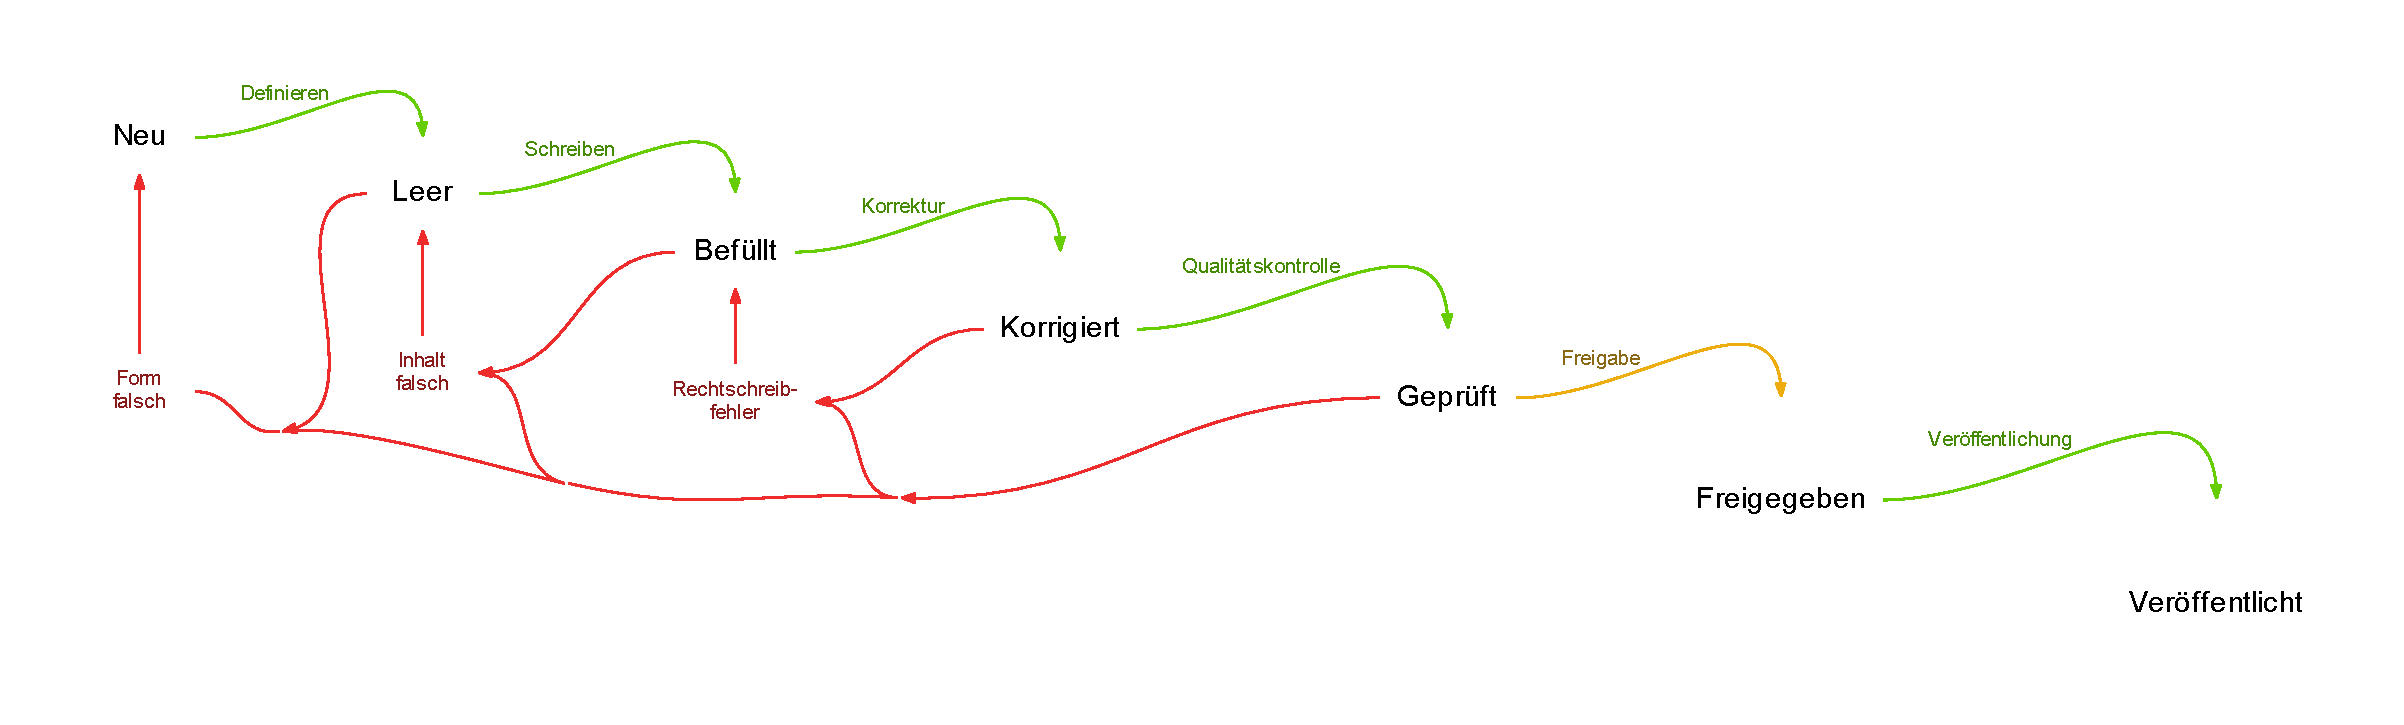
\includegraphics[width=\textwidth]{media/chart-4.pdf}
\end{center}
\caption{Operationen bei der Erstellung von Texten mit Qualitätskontrolle}
\label{chart:4}
\end{figure}